% =============================================================================
% COPYRIGHT AND DISCLAIMER
% =============================================================================
% This file is provided as a convenience template for competition participants.
% By using it, you accept full responsibility for compliance with all applicable
% copyright, licensing, and usage rules of the Association for Computing
% Machinery (ACM) and of any LaTeX packages you load (including, without
% limitation, the "acmart" document class and related ACM materials).
%
% Consult ACM's official publication, template, and copyright policies before
% using this setup for any purpose other than this competition. Do not assume
% that this template may be reused, redistributed, or submitted elsewhere
% without independently verifying ACM's current rules.
%
% Use of the "acmart" class, the "sigconf" option, or ACM-style formatting in
% this template does NOT mean that this report, this competition, its organizers,
% or any resulting PDF is sponsored, endorsed, affiliated with, or published by
% ACM. ACM trademarks and branding remain the property of ACM.
%
% Template packages live in preamble.tex.
% Citations live in main.bib. Edit this file with your paper content.
% =============================================================================

\documentclass[sigconf]{acmart}
% =============================================================================
% Template setup — participants normally do not edit this file.
% Author content belongs in main.tex; citations belong in main.bib.
% \documentclass lives in main.tex so Overleaf does not treat this file as root.
% =============================================================================

% --- Competition / non-ACM-submission friendly rights metadata -------------
\setcopyright{none}
\settopmatter{printacmref=false}
\acmConference[Kaggle Competition]{Filament Segmentation Challenge}{2026}{\href{https://www.kaggle.com/competitions/filament-segmentation-2026}{kaggle.com/competitions/filament-segmentation-2026}}
\acmBooktitle{Competition Report}
\acmDOI{}
\acmISBN{}

% --- Author guidance text --------------------------------------------------
% \guide{...} is gray italic while \guideStyletrue; omitted from the PDF if false.
% Flip the switch in main.tex after % =============================================================================
% Template setup — participants normally do not edit this file.
% Author content belongs in main.tex; citations belong in main.bib.
% \documentclass lives in main.tex so Overleaf does not treat this file as root.
% =============================================================================

% --- Competition / non-ACM-submission friendly rights metadata -------------
\setcopyright{none}
\settopmatter{printacmref=false}
\acmConference[Kaggle Competition]{Filament Segmentation Challenge}{2026}{\href{https://www.kaggle.com/competitions/filament-segmentation-2026}{kaggle.com/competitions/filament-segmentation-2026}}
\acmBooktitle{Competition Report}
\acmDOI{}
\acmISBN{}

% --- Author guidance text --------------------------------------------------
% \guide{...} is gray italic while \guideStyletrue; omitted from the PDF if false.
% Flip the switch in main.tex after % =============================================================================
% Template setup — participants normally do not edit this file.
% Author content belongs in main.tex; citations belong in main.bib.
% \documentclass lives in main.tex so Overleaf does not treat this file as root.
% =============================================================================

% --- Competition / non-ACM-submission friendly rights metadata -------------
\setcopyright{none}
\settopmatter{printacmref=false}
\acmConference[Kaggle Competition]{Filament Segmentation Challenge}{2026}{\href{https://www.kaggle.com/competitions/filament-segmentation-2026}{kaggle.com/competitions/filament-segmentation-2026}}
\acmBooktitle{Competition Report}
\acmDOI{}
\acmISBN{}

% --- Author guidance text --------------------------------------------------
% \guide{...} is gray italic while \guideStyletrue; omitted from the PDF if false.
% Flip the switch in main.tex after \input{preamble}.
%
% Do not use \guide{...} for \email{...}.
\usepackage{xcolor}
\newif\ifguideStyle
\guideStyletrue
\newcommand{\guide}[1]{%
  \ifguideStyle
    {\color{gray!65}\itshape #1}%
  \fi
}

% --- Math ------------------------------------------------------------------
% Do NOT load amssymb (or amsfonts): acmart already loads newtxmath, which
% defines the same symbols (e.g. \Bbbk) and causes a conflict on Overleaf.
% amsmath is already provided by acmart; mathtools extends it.
\usepackage{mathtools}

% --- Figures ---------------------------------------------------------------
% graphicx is already loaded by acmart
\usepackage{subcaption}

% --- Tables ----------------------------------------------------------------
% booktabs is already loaded by acmart
\usepackage{tabularx}
\usepackage{multirow}

% --- Bibliography style is set in main.tex (ACM-Reference-Format) ----------
.
%
% Do not use \guide{...} for \email{...}.
\usepackage{xcolor}
\newif\ifguideStyle
\guideStyletrue
\newcommand{\guide}[1]{%
  \ifguideStyle
    {\color{gray!65}\itshape #1}%
  \fi
}

% --- Math ------------------------------------------------------------------
% Do NOT load amssymb (or amsfonts): acmart already loads newtxmath, which
% defines the same symbols (e.g. \Bbbk) and causes a conflict on Overleaf.
% amsmath is already provided by acmart; mathtools extends it.
\usepackage{mathtools}

% --- Figures ---------------------------------------------------------------
% graphicx is already loaded by acmart
\usepackage{subcaption}

% --- Tables ----------------------------------------------------------------
% booktabs is already loaded by acmart
\usepackage{tabularx}
\usepackage{multirow}

% --- Bibliography style is set in main.tex (ACM-Reference-Format) ----------
.
%
% Do not use \guide{...} for \email{...}.
\usepackage{xcolor}
\newif\ifguideStyle
\guideStyletrue
\newcommand{\guide}[1]{%
  \ifguideStyle
    {\color{gray!65}\itshape #1}%
  \fi
}

% --- Math ------------------------------------------------------------------
% Do NOT load amssymb (or amsfonts): acmart already loads newtxmath, which
% defines the same symbols (e.g. \Bbbk) and causes a conflict on Overleaf.
% amsmath is already provided by acmart; mathtools extends it.
\usepackage{mathtools}

% --- Figures ---------------------------------------------------------------
% graphicx is already loaded by acmart
\usepackage{subcaption}

% --- Tables ----------------------------------------------------------------
% booktabs is already loaded by acmart
\usepackage{tabularx}
\usepackage{multirow}

% --- Bibliography style is set in main.tex (ACM-Reference-Format) ----------


% Guide styling: \guideStyletrue = show gray italic hints; \guideStylefalse = omit them
\guideStylefalse
% \guideStyletrue

\begin{document}

\title[Filament Segmentation with a DINOv3 Ensemble]{Solar Filament Instance Segmentation with a DINOv3 Ensemble and Learned Candidate Selection}  % Replace this with your title
\subtitle{A Solution to the Solar Filament Segmentation Challenge 2026} % DO NOT CHANGE


\author{Yuya Kaneta} 
\affiliation{%
  \institution{Independent Researcher}
  \city{Tokyo}
  \country{Japan}
}
\email{yucho147@gmail.com}

% \author{\guide{Second Author}}
% \affiliation{%
%   \institution{Affiliation to be supplied}  % <- Optional (remove if you are not currently affiliated with any institute)
%   \city{City to be supplied}
%   \country{Country to be supplied}
% }
% \email{second.author@example.com}  % <- Replace with your own email

\begin{abstract}
    This report describes our solution to the Solar Filament Segmentation Challenge~2026, a Kaggle competition on automatic segmentation of solar filaments in GONG H-$\alpha$ observations. Our submission averages ten fine-tuned DINOv3 models and selects connected components with a learned scoring model. It achieved a public panoptic quality (PQ) score of 0.38, the same as our earlier five-model submission. On a two-model proxy evaluated across 547 development images, the selector improved PQ over fixed post-processing by 0.0083 (95\% paired time-block interval: 0.0037--0.0130). This proxy does not directly evaluate the submitted ten-model ensemble, and the development folds informed model selection. On an RTX 3090, inference from the saved weights reproduced the submitted CSV byte-for-byte; the original training process was not reproduced.
\end{abstract}

\maketitle

\ifguideStyle
\noindent{\color{gray!65}\itshape
Guide mode is on.}
\par\medskip
\fi

\guide{Please limit your report to four (4) pages, excluding the Acknowledgment and References sections. Throughout this document, please follow these considerations: 
\begin{itemize}
    \item Do not alter any text that is currently in black color (except for the emails under authors' name).
    \item Replace all gray text with your own.
    \item When you are done with the report, please replace \texttt{\textbackslash guideStyletrue} with \texttt{\textbackslash guideStylefalse}, to remove any gray text. Alternatively, you can remove any text wrapped in \texttt{\textbackslash guide\{\}},
    \item Be as succinct as possible, and only provide details regarding your own work. For example, there is no need to discuss what solar filaments are, or why filament segmentation matters.
    \item If you must, you can add extra sections.
\end{itemize}}


% ==================================== %
%              INTRODUCTION            %
% ==================================== %
\section{Introduction}
    This report goes over the details of our submitted solution to the Solar Filament Segmentation Challenge~2026 \cite{filament-segmentation-2026}. The challenge, launched on July~10,~2026, is organized by the Earth-Space AI Research (ESAIR) Lab\footnote{\href{https://www.esairlab.com/home}{www.esairlab.com/}}. This challenge utilizes the MAGFiLO dataset for evaluation of the segmentation algorithms \cite{ahmadzadeh2024dataset}. We address instance segmentation from the provided H-$\alpha$ image alone, respecting the multiple annotation sets in evaluation. Our selected submission is the learned-selector candidate C; a fixed-rule alternative A2 is retained for comparison.


% ==================================== %
%              METHODOLOGY             %
% ==================================== %
\section{Methodology}\label{sec:methodology}
The training set comprises 707 physical images and the test set 180 images. We set aside 108 final-holdout images and a 52-image buffer; the remaining 547 images form five outer folds using 27-day blocks and a 14-day temporal purge. Each outer-training set has an inner tuning split. The outer folds were repeatedly inspected during development; reported results are therefore exploratory. The final holdout was not used to select this submission.

\textbf{Inputs and targets.} Images are read as 8-bit grayscale at their original $2048\times2048$ resolution and scaled to $[0,1]$. For each annotation set, the polygons are rasterized and combined into one foreground mask. The target at each pixel is the mean of those binary masks across annotation sets. This soft target retains annotation disagreement rather than treating any one annotator as uniquely correct. A target value of $1/3$, for example, means that one of three sets includes that pixel; it is not a claim about the probability of physical presence.

\textbf{Model and training.} We fine-tune the pretrained DINOv3 ViT-L/16 encoder~\cite{dinov3} with a high-resolution decoder using native $512\times512$ crops. The grayscale input is replicated into three channels and normalized using the encoder's pretrained configuration. Four intermediate transformer outputs are concatenated and projected; a parallel convolutional branch preserves high-resolution image features. The decoder progressively upsamples and combines these features to produce one foreground logit per input pixel. The separate high-resolution branch is intended to retain narrow filament detail that can be lost at the transformer's 16-pixel patch scale.

Training uses binary cross-entropy plus soft Dice loss, AdamW, batch size 8, spatial flips and rotations, and weak brightness/contrast augmentation. A batch includes three overlapping crops from one image and five crops sampled separately; sampling favors foreground while retaining background examples. Encoder and decoder peak learning rates are $6\times10^{-5}$ and $3\times10^{-4}$, with encoder layer-wise decay 0.9 and weight decay $10^{-4}$. The schedule warms up for 600 updates and follows a 12,000-update cosine schedule. For seed 42, inner validation selects 10,500/7,500/7,000/7,500/8,500 refit updates for folds 0--4, respectively. We retain exponential moving averages (EMA) of the weights with maximum decay 0.999. EMA smooths a single training trajectory; it is not the same operation as averaging independent models.

\textbf{Inference.} Each of ten fold models (five per seed) processes overlapping native-resolution tiles (50\% overlap, or stride 256) using three views: unmodified, horizontally flipped, and vertically flipped. Inverse-transformed tile probabilities are combined with uniform weights; the five probability maps of each seed are averaged, and the two seed-level maps are then averaged with equal weights (a ten-model equal-weight mean, computed in float32). Overlap is intended to reduce dependence on a pixel's position within an individual crop; its effect was not isolated in this final configuration. Figure~\ref{fig:pipeline} depicts the pipeline for one seed. On an RTX 3090 the ten models required 98 minutes for 180 images (two passes of about 16.3\,s per image) and 7.6 GB peak GPU memory per five-model pass (running all ten together is estimated at about 14 GB, unmeasured); these figures exclude transfer and setup. The fine-tuned weights total 12.2 GB.

\textbf{Two seeds.} The second seed (43) uses the same configuration, folds, and EMA decay (0.999) as the first (42); only the random seed differs. Seed-43 folds 0 and 1 were retrained after the first runs were lost before retrieval, and the manifest of seed-43 fold 3 was lost and reconstructed (Section~\ref{sec:evaluation}). Training steps per fold were fixed by the inner selection of each seed (7000--10500 for seed 42; 5000--9000 for seed 43). Runs with the same seed and configuration differ across hosts: single-model outer PQ differed by up to 0.013 per fold between two same-seed runs, so differences between seeds are not interpreted as seed effects.

\begin{figure}[t]
\centering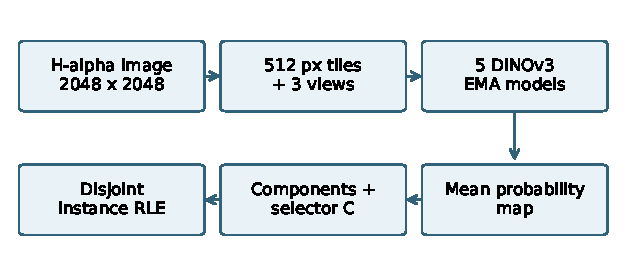
\includegraphics[width=\columnwidth]{pipeline.pdf}
\caption{Inference pipeline (shown for one seed's five fold models). The submitted ten-model candidate averages two such five-model maps with equal weights; C and A2 both start from the same averaged probability map.}\label{fig:pipeline}
\end{figure}

\textbf{Candidate selection.} C extracts 8-connected components from probability $>0.4$ with area at least 100 pixels. Two gradient-boosted regressors estimate (i) the fraction of annotation sets matched at intersection over union (IoU) $>0.5$ and (ii) the IoU conditional on a match. A component is retained when their product is at least 0.25. Eleven label-free descriptors include area, probabilities, shape, location, and relationships to components at other thresholds. The selector is trained on 496 image-model pairs corresponding to 363 development images predicted by their inner models without training on those images. A2 instead keeps components of area at least 400 pixels and peak probability at least 0.995. Figure~\ref{fig:examples} illustrates submitted C predictions; test ground truth is unavailable.

The component relationships are computed at thresholds 0.30, 0.40, 0.50, 0.60, 0.70 and 0.85. The features comprise log area, threshold, peak/mean/standard deviation of probability, area relative to the parent, number of children, largest-child area ratio, bounding-box aspect ratio and fill, and normalized radial position. Both regressors use histogram gradient boosting (maximum depth 3, 200 iterations, learning rate 0.05, minimum leaf size 20). The conditional-IoU regressor is fitted only on candidates with a match. The product estimates expected matched IoU across annotation sets, combining whether a candidate is drawn with how well its shape agrees; it is a decision score, not a calibrated pixel probability. We select at the 0.40 level only, so outputs are disjoint and exported as compressed COCO RLE. The operating threshold was selected on inner predictions; the proxy results below do not use test labels.

\textbf{Selector for the ten-model candidate.} The selector is retrained on the mean of the seed-42 and seed-43 inner-model probabilities of the inner tuning images (five folds, 496 rows, 363 distinct images), with $\tau=0.25$ chosen by cross-fitting grouped by physical image (the original fold-wise choice also gives 0.25). Test images and the final holdout are not used.

\begin{figure}[t]
\centering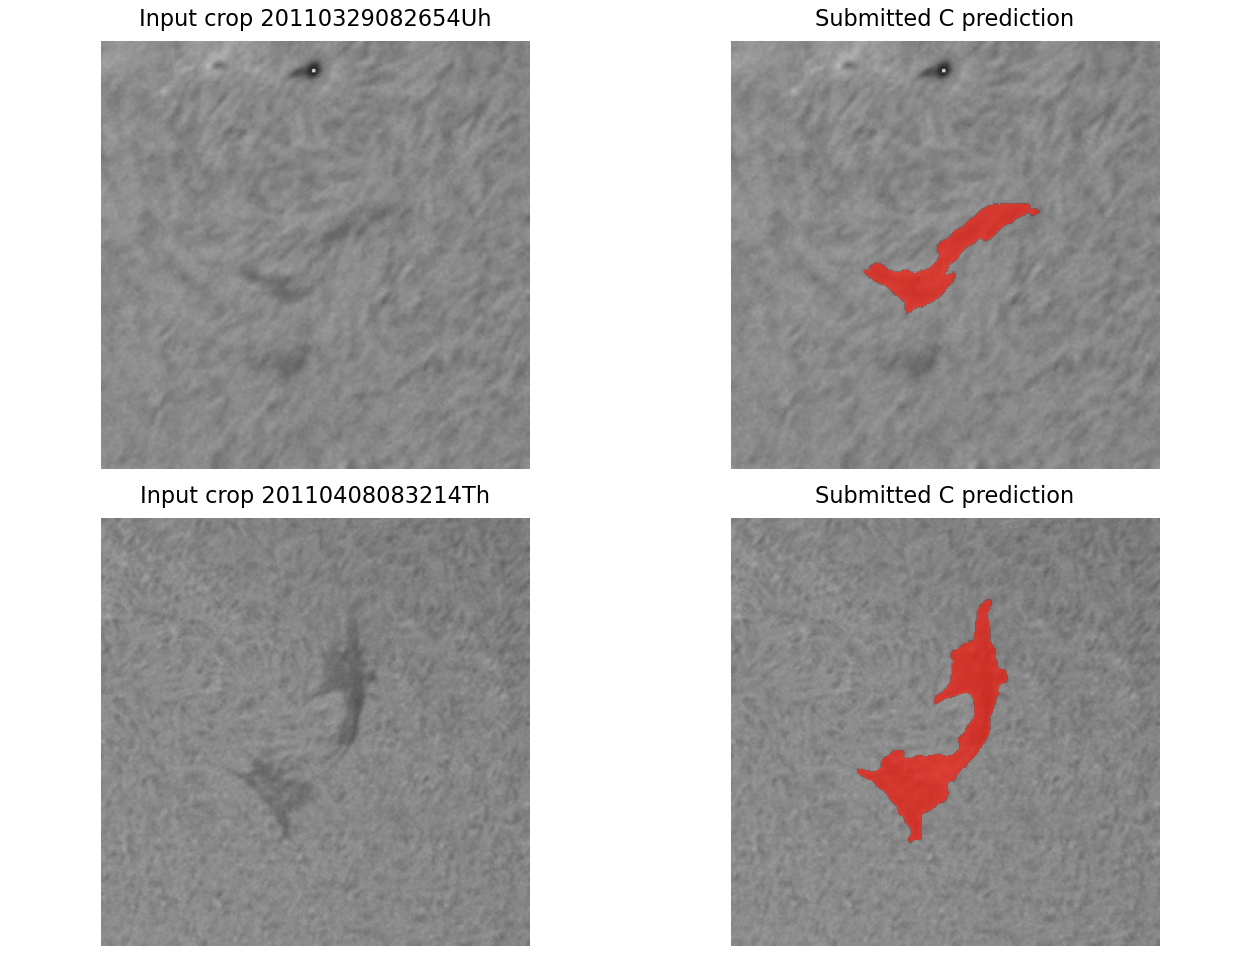
\includegraphics[width=0.91\columnwidth]{examples.png}
\caption{Crops from two test inputs and submitted C masks (red); examples are descriptive, not accuracy estimates. Test labels are unavailable. Images: MAGFiLO/GONG competition data.}\label{fig:examples}
\end{figure}

% ==================================== %
%              EVALUATION              %
% ==================================== %
\section{Evaluation}\label{sec:evaluation}
\textbf{Metric and protocol.} For every annotation set, the public scorer compares predictions with ground truth: a prediction matches a ground-truth instance when IoU $>0.5$; matched IoUs, true positives (TP), false positives (FP), and false negatives (FN) are pooled for panoptic quality (PQ)~\cite{kirillov2019}. Segmentation quality (SQ) is the mean IoU of matched instances, and recognition quality (RQ) summarizes detection; PQ is their product. Unless stated otherwise, uncertainty intervals are 95\% paired time-block resampling intervals.

The submitted ten-model average (and the earlier five-model average) cannot be scored as an unseen-image prediction on the development images because several fold models trained on each image. As a proxy, we average two independently trained models of the same fold, neither trained on its evaluation images. For each fold, selector training is restricted to its outer-training images. The same fixed C and A2 procedures are applied to the outer evaluation images. Two proxies are used: P-old (seed-42 ordinary training plus a seed-42 EMA run, i.e.\ two runs of the same seed) and P-new (seed-42 EMA plus seed-43 EMA, i.e.\ two seeds, the closest analogue of the final candidate).

\begin{table}[t]\centering\small
\begin{tabular}{lrrrrrr}\toprule
 & PQ & SQ & RQ & TP & FP & FN\\\midrule
A2 & .4299 & .6839 & .6287 & 3928 & 2081 & 2559\\
C & .4415 & .6855 & .6441 & 4005 & 1944 & 2482\\\bottomrule
\end{tabular}
\caption{Earlier same-seed proxy (P-old), pooled over 547 development images and 891 annotation sets. C$-$A2 PQ is $+0.0116$ (95\% paired block interval $[0.0076,0.0157]$); all five folds are positive. This estimate is subject to indirect information flow: the selector's training rows come from other folds' inner models, which were trained on 38--77 of each evaluated fold's images; the effect on this number is unmeasured.}\label{tab:results}
\end{table}

\begin{table}[t]\centering\small
\begin{tabular}{lrrrrr}\toprule
Outer fold & 0 & 1 & 2 & 3 & 4\\\midrule
C$-$A2 PQ & .0055 & .0048 & .0190 & .0168 & .0108\\\bottomrule
\end{tabular}
\caption{Earlier same-seed proxy (P-old): per-fold PQ differences. Fold sample sizes and annotation counts differ; the pooled difference is computed from pooled counts rather than the mean of these five values.}\label{tab:folds}
\end{table}

\textbf{Evaluation correction.} Our first cross-fold selector evaluation mistakenly included some evaluation images in selector training; its $+0.0158$ estimate is invalid. The corrected comparison in Table~\ref{tab:results} excludes each evaluated fold's images from selector training. Training each selector only on its own inner tuning set gives a smaller pooled gain, $+0.0076$ for the two-model proxy. Neither evaluation directly measures the submitted five-model average.

\textbf{Indirect information flow and its audit.} In the $+0.0116$ evaluation the selector for outer fold $k$ is trained on rows produced by the inner models of the other four folds. Those inner models were trained on 38--77 images of fold $k$'s evaluation set (50/38/58/61 for fold 0, 66/56/59/59 for fold 1, 70/74/77/67 for fold 2, 53/68/68/51 for fold 3, 71/58/46/65 for fold 4), so evaluation labels can reach the selector indirectly through the image model; the size of this effect is \emph{not measured}, and the $+0.0116$ should be read as possibly optimistic. The own-inner-tune evaluation ($+0.0076$, 95\% block interval $[0.0043,0.0108]$) separates both the image model and the selector from the evaluated images (inner-model training set, tuning set and evaluation set are disjoint), but each selector sees only about 100 images, making the estimate less precise and not directly representative of the final selector. A second, separate issue was that the threshold $\tau$ was chosen by cross-fitting over original inner folds, so the same physical image could lie on both sides (11--38 images per held-out group; 55/46/58/55/27 of 101/96/91/106/102 for the final selector). Re-choosing $\tau$ with groups by physical image or by 27-day block (with a 14-day exclusion) gives a two-model proxy gain of $+0.0094$ $[0.0052,0.0134]$ and $+0.0093$ $[0.0051,0.0134]$, i.e.\ about $+0.009$, and the final selector's $\tau$ is 0.25 in every variant, so the submitted selector is unchanged. This re-selection does not remove the indirect flow through the image models, which remains in the $+0.009$ figures. The evaluated folds have been referenced repeatedly, and no evaluation of the five-model average on unseen development images was possible.

\textbf{Analysis and limitations.} In the proxy, the improvement is mainly associated with detection quality (RQ .6287 to .6441 and FP $-137$), while segmentation quality changes from .6839 to .6855. Matched-pair mean IoU is .684 versus .686, and mean Dice is .809 versus .810; unmatched objects are not included in these shape statistics. Split ground-truth instances decrease from 207 to 166, while merged predictions remain at 80, under a separate 50\% overlap convention. The two Kaggle submissions received public scores 0.37 (A2) and 0.38 (C), rounded to two decimals; A2 used MPS fp32 and C CUDA bf16, so the difference is not solely attributable to selection. The public portion covers only part of the test set and private performance remains unknown.

\textbf{Failure modes and interpretation.} The proxy contains 6,487 ground-truth instances across annotation sets. Under A2, 1,584 have no overlapping prediction, while 624 have only weak overlap and 207 meet our separate split criterion. C cannot recover a structure absent from the candidate components. Lower-threshold candidates or a model trained to preserve faint structures could improve recall, but would require validation against additional false positives. Its main effect is choosing which existing components to retain: FP falls from 2,081 to 1,944 while TP rises from 3,928 to 4,005. The split count uses the following descriptive convention: an unmatched ground-truth instance is split when at least two predictions each have more than half their area inside it and jointly cover over half of it. These values are not independent per-object uncertainty estimates.

For a within-run EMA comparison, the five single-model outer evaluations yield pooled PQ 0.4188 with the ordinary weights and 0.4236 with EMA, a difference of $+0.0047$ with paired block interval $[0.0008,0.0087]$. Four folds improve and one worsens. These numbers compare single-model predictions and do not measure the submitted five-model ensemble. They motivated retaining EMA but do not establish that EMA is always beneficial.

\textbf{Ten-model candidate: what the development images show.} The numbers below are two-model proxies (not the ten-model average), pooled over 547 images with paired time-block 95\% intervals, using for each fold a selector trained only on that fold's own inner tuning images. (i) Adding a second seed to one EMA series (P-new versus seed-42 EMA alone) gains $+0.0047$ $[0.0014,0.0080]$ PQ with A2 (positive in 5/5 folds) and $+0.0047$ $[0.0010,0.0085]$ with C (4/5 folds). (ii) P-new versus P-old gains $+0.0059$ $[0.0012,0.0108]$ with A2 and $+0.0066$ $[0.0016,0.0116]$ with C, but this depends on fold 2: without it the gains are $+0.0016$ and $+0.0005$, with intervals that include zero, and P-old is a same-seed pair. (iii) On P-new, C$-$A2 is $+0.0083$ $[0.0037,0.0130]$ (5/5 folds). (iv) Retraining the selector on seed-averaged probabilities instead of reusing the seed-42 selector adds only $+0.0010$ $[-0.0019,0.0041]$ and is not claimed as an improvement. (v) Seed 43 alone is slightly lower than seed 42 alone ($-0.0045$ $[-0.0091,0.0001]$ with A2), within run-to-run variation. These numbers do not establish that the ten-model average beats the five-model average; the public score is identical (0.38).

\textbf{Extensions evaluated after the candidate was frozen (none adopted).} On the same 547 development images (out-of-fold predictions, selector C, paired time-block intervals; fold models were not re-tuned, so these are exploratory), we tested: a third seed (+0.0010 $[-0.003,+0.005]$ over two seeds on three folds); a logit average of the two DINOv3-L seeds with an EfficientNetV2-S U-Net ($-0.0043$ $[-0.0086,-0.0002]$, worse on all five folds); a pixel-level learned stacker over nine models with image features (worse on both folds tested); and an instance-level refiner on rotated $384\times128$ crops ($+0.0008$ $[-0.0021,+0.0034]$ on top of C). We therefore keep the ten-model C unchanged.

\textbf{Provenance and reproducibility.} For all ten weights, the training images share no image with the fold's evaluation images, the final holdout, or the test set, and the SHA-256 of nine weight files matches its original manifest. The seed-43 fold-3 manifest and training logs were lost with a rented machine; its manifest was reconstructed from the fold-2 record with the fold, training images, and the SHA-256 of the retrieved file substituted, so that match is self-referential and is not evidence that the file equals the original training output. Seed-43 folds 0 and 1 are retrained runs (their first runs were lost); the training-time code commit is unavailable for all weights. On a CUDA RTX 3090 (torch 2.8.0+cu128, CUDA 12.8), running the candidate notebook in inference mode from the ten weight files reproduced all 180 probability hashes of both seed-level maps and the ten-model map and the submitted CSV byte-for-byte (1207 rows, 177 of 180 images). This verifies that the saved files reproduce the submission on this GPU class; it is not a reproduction of the training process, which cannot be reproduced exactly (same-seed runs differ). Other devices, drivers, or precisions may give slightly different probabilities. Three test images receive no C prediction in either version. The outer folds have been inspected repeatedly, and the uncertainty intervals measure evaluation-image variability rather than all model-selection and training uncertainty. Redistribution conditions and hosting of the fine-tuned weights (12.2 GB) remain unresolved.
% ==================================== %
%            ACKNOWLEDGMENT            %
% ==================================== %
\section{Acknowledgment}\label{sec:acknowledgment}
    % Do not change
    The organization of the Filament Segmentation Challenge 2026 is partially supported by the U.S. National Science Foundation (NSF) under Grant No. 2209912 and 2433781, directorate for Computer and Information Science and Engineering (CSE), and Office of Advanced Cyberinfrastructure (OAC), and Grant No. 2511630, AST Division Of Astronomical Sciences and MPS Directorate for Mathematical and Physical Sciences.

    The Filament Segmentation Challenge 2026 is sponsored by the U.S. National Science Foundation (NSF) National Solar Observatory (NSO). 

    This work utilizes GONG data obtained by the NSO Integrated Synoptic Program, managed by the National Solar Observatory, which is operated by the Association of Universities for Research in Astronomy (AURA), Inc. under a cooperative agreement with the National Science Foundation and with contribution from the National Oceanic and Atmospheric Administration. The GONG network of instruments is hosted by the Big Bear Solar Observatory, High Altitude Observatory, Learmonth Solar Observatory, Udaipur Solar Observatory, Instituto de Astrofísica de Canarias, and Cerro Tololo Interamerican Observatory.

\bibliographystyle{ACM-Reference-Format}
\bibliography{main}

\end{document}
